\documentclass{rapportECL}

\usepackage{minted}
%https://www.overleaf.com/learn/latex/Code_Highlighting_with_minted

%https://www.overleaf.com/latex/examples/source-code-highlighting-with-minted-in-latex/qphhfvnsddbs


 
%\usepackage{listingsutf8} %Display code in LaTeX, using the lstlisting environment
% https://tex.stackexchange.com/questions/312429/an-error-appears-saying-that-utf8-and-listing-are-not-compatible?rq=1


\title{Méthode Mixte : classification et analyse factorielle} %Titre du fichier

\begin{document}

%----------- Informations du rapport ---------

\titre{Méthode Mixte : classification et analyse factorielle} %Titre du fichier .pdf
\UE{UE INF a 4-EG} %Nom de la UE
\sujet{Analyse de Données} %Nom du sujet

\enseignant{Emmanuel \textsc{Dellandréa}} %Nom de l'enseignant

\eleves{Bruno \textsc{Moreira Nabinger} \\
		Clément \textsc{Vinot} } %Nom des élèves

%----------- Initialisation -------------------
        
\fairemarges %Afficher les marges
\fairepagedegarde %Créer la page de garde
\tabledematieres %Créer la table de matières

%------------ Corps du rapport ----------------


\section{Introduction} 
%slide 66-67/72
Comme vu en cours, les méthodes d’analyse factorielle sont bien adaptées à l’exploration de tableaux de données de taille importante, mais une seule partie de l'information est représentée et parfois elle est trop complexe. C'est à ce moment-là que l'on peut recourir à une des techniques de classification non-supervisée pour réaliser la compréhension de la structure des donnés et faciliter l'interprétation des résultats. On a donc une démarche combine. 

L'objectif général de ce 

\section{Cahier des charges}

\section{Principe des Solutions}
%slide 68/72
Le principe de la classification mixte repose sur trois étapes :
\begin{itemize}
    \item analyse factorielle ;
    \item classification à partir des facteurs ;
    \item positionnement des classes dans le plan factoriel.
\end{itemize}
%slide 69-70/72
La premier étape consiste dans la réalisation de l'analyse factorielle à partir des donnés, ce qui nous fournit les facteurs qui résument au mieux l'information contenue dans les donnés. Si $p$ est le nombre de variables des donnés de départ, la analyse factoriel nous permet d'obtenir $q$ facteurs, avec $q \ll  p$, qui contient la plus part de l'information portée par les $p$ variables.
%slide 3/72 70-71/72
La classification non-supervisée est destinée à produire des groupements de lignes ou de colonnes d'un tableau.

"On cherche donc à les mettre en évidence
par des représentations des classes
d’éléments sous forme de partitions (ou
hiérarchies de partitions)" %slide 4/72

"Un des avantages des méthodes de
classification est de mettre en évidence des
classes souvent plus faciles à décrire
automatiquement que les axes factoriels" %slide 6/72

"La classification réalisée à partir des q facteurs
peut reposer sur des méthodes de centres
mobiles ou de classification ascendante
hiérarchique" %slide 70-71/72

"La classification offre la possibilité de projeter les centres des 
classes sur ces plans, et d’indiquer également la classe
d’appartenance des éléments (couleurs différentes par exemple)"%slide 70-71/72


Des modules différents ont été développés pour chacune des 

\section{Implementation}

L'implementation du programme a été faite avec la langage Python 3.7. Le documentation a été fait en utilisant docstrings et des commentaires. On a aussi fait le design du code de tel façon  à aider la compréhension, en choisissant les nome des variables, attributs et méthodes qui explicitent la solution. Quelques méthodes ont été nommés d'après les fichiers disponibles dans la plateforme Pédagogique.

L'archive BE3-remarques-fusion.pdf disponibles dans la plateforme Pédagogique a été utilise pour réaliser quelques optimisations dans le code.

Le code est montré dans le topique suivant:

Figure \ref{fig: Label diagramme_des_inerties}.

%------ Pour insérer et citer une image centralisée -----
\insererfigure{img/diagramme_des_inerties_acp.jpeg}{8cm}{Diagramme des inerties : ACP}{Label diagramme_des_inerties}
% Le premier argument est le chemin pour la photo
% Le deuxième est la hauteur de la photo
% Le troisième la légende
% Le quatrième le label

Cette méthode mixte devra être réalisée pour quatre combinaisons :
- ACP + CAH
- ACP + centres mobiles
- ACM + CAH
- ACM + centres mobiles



\section{Démarche et analyse des résultats}

\subsection{ACP/ACM + CAH}
%Classification ascendante hiérarchique

\subsubsection{Démarche}

La démarche pour les deux méthodes consiste à appliquer respectivement une ACP, après normalisation, et une ACM aux données, après mise en classe, puis de classer les résultats par une méthode de Classification ascendante hiérarchique (CAH).

Les données utilisées dans l'exemple donné en graphique sont issues de la base "populations".

Ces données étant quantitatives, l'ACP peut s'appliquer directement, mais il faut réaliser une mise en classe pour obtenir un tableau disjonctif complet (TDC) et réaliser l'ACM. L'ACM correspont à une Analyse factoriel des correspondances binaires (AFC) d'un TDC, qui n'est pas traité dans ce rapport.

En suite, on utilise la méthode de Classification ascendante hiérarchique (CAH). Tout d'abord, on réalise la construction de l'arbre hiérarchique par agrégations successives de deux éléments en utilisant la fonction \textit{linkage} issue du module \textit{scipy.cluster.hierarchy (Hierarchical clustering)}. Cette fonction admet différentes méthodes pour calculer la distance entre des éléments.




Une fois ces méthodes de factorisation appliquées, on peut appeler la fonction \textit{linkage} issue du module \textit{scipy} pour réaliser une classification par la méthode des centres mobiles.

Dans les exemples de résultats ci-dessous, on a choisi respectivement un nombre de classes $k = 3$ et $5$ pour l'ACM et l'ACP arbitrairement en fonction du nombre de données pour obtenir des graphiques visibles tout en observant l'efficacité de la méthode.

Les étoiles représentent les centres, et les couleurs l'appartenance à la classe de chaque point.

\begin{figure}[!htb]
        %\captionsetup[subfigure]{labelformat=empty}
        \begin{subfigure}[b]{0.45\textwidth}
            \centering
            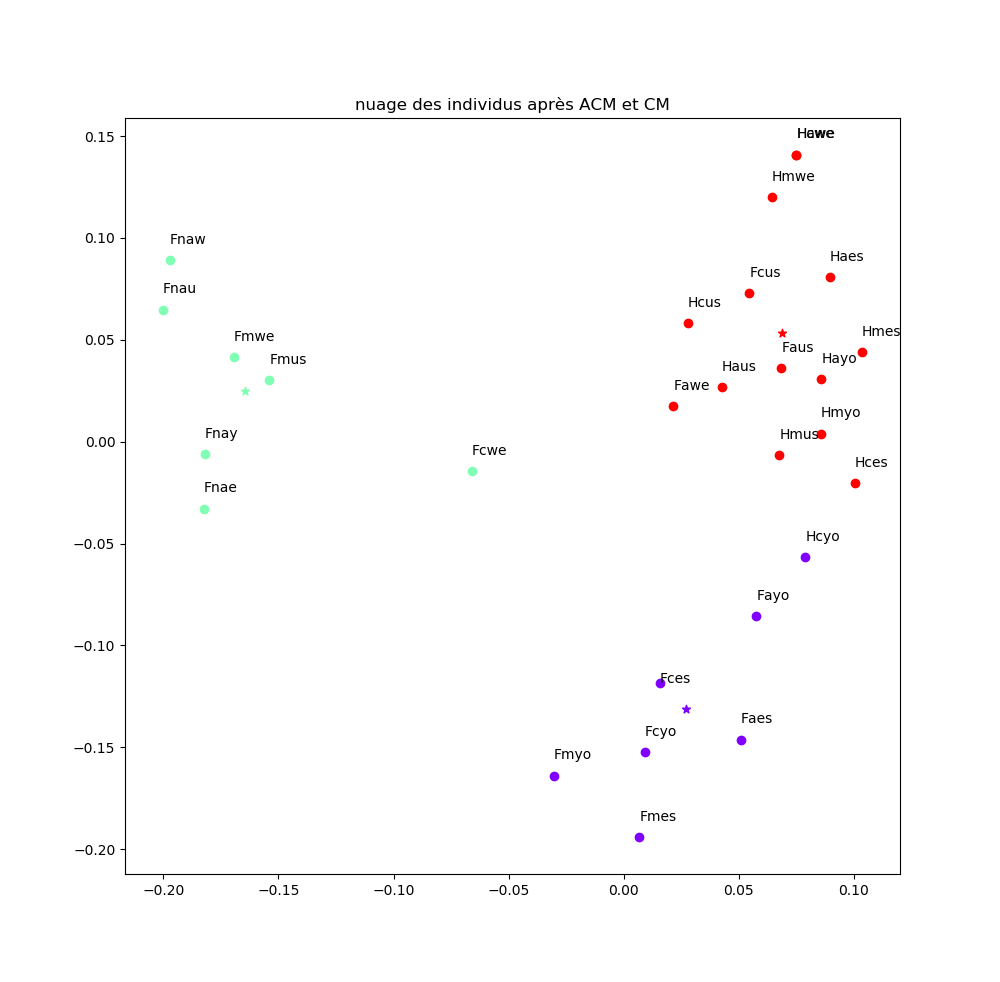
\includegraphics[width=0.9\textwidth]{img/Individus_ACM-CM.png}
            \caption{ACM + CM : Projection des individus}
            \label{Label_Individus_ACM-CM.png}
        \end{subfigure}
        \begin{subfigure}[b]{0.45\textwidth}
            \centering
            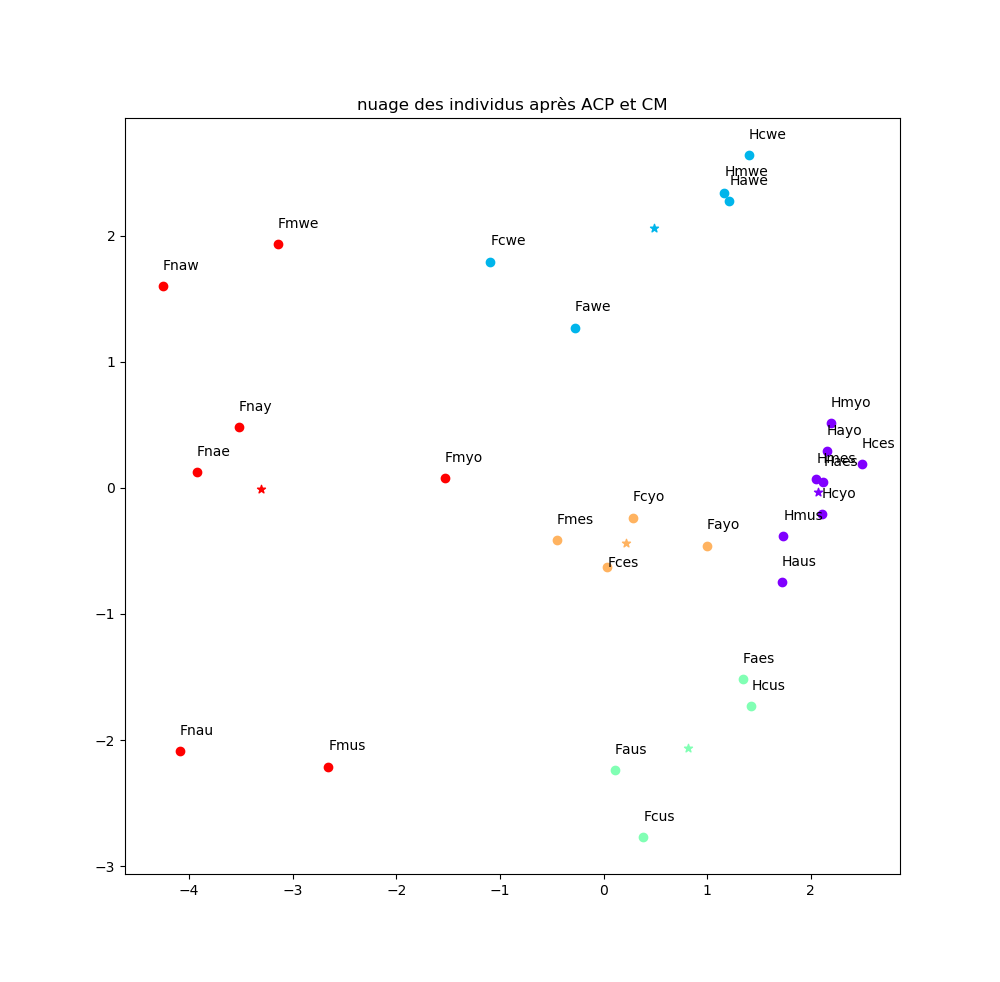
\includegraphics[width=0.9\textwidth]{img/Individus_ACP-CM.png}
            \caption{ACP + CM : Projection des individus}
            \label{Label_Individus_ACP-CM.png}
        \end{subfigure}
        \caption{Résultats pour l'ACP/ACM + CM : Projection des individus}
        \label{Label_Individus_ACP_ACM-CM.png}
    \end{figure}
    
    \begin{figure}[!htb]
        %\captionsetup[subfigure]{labelformat=empty}
        \begin{subfigure}[b]{0.45\textwidth}
            \centering
            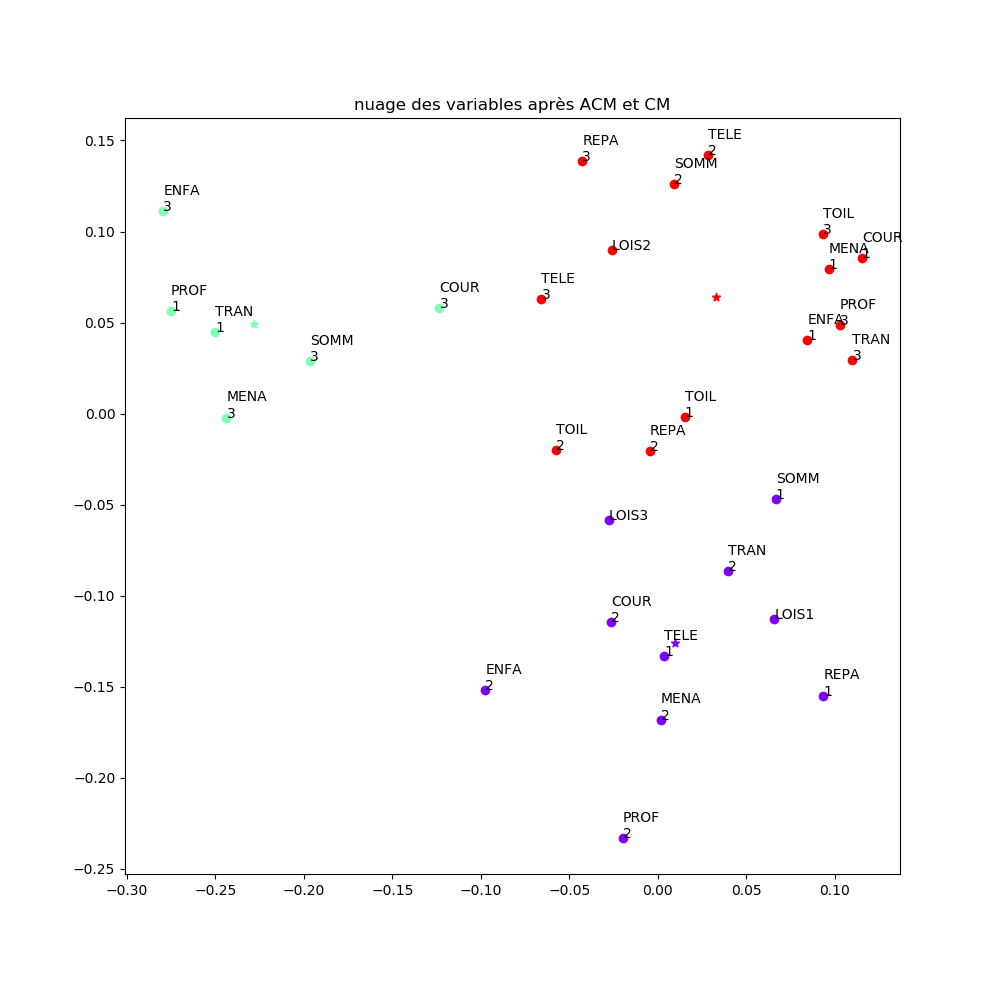
\includegraphics[width=0.9\textwidth]{img/Variables_ACM-CM.png}
            \caption{ACM + CM : Projection des variables}
            \label{Label_Variables_ACM-CM.png}
        \end{subfigure}
        \begin{subfigure}[b]{0.45\textwidth}
            \centering
            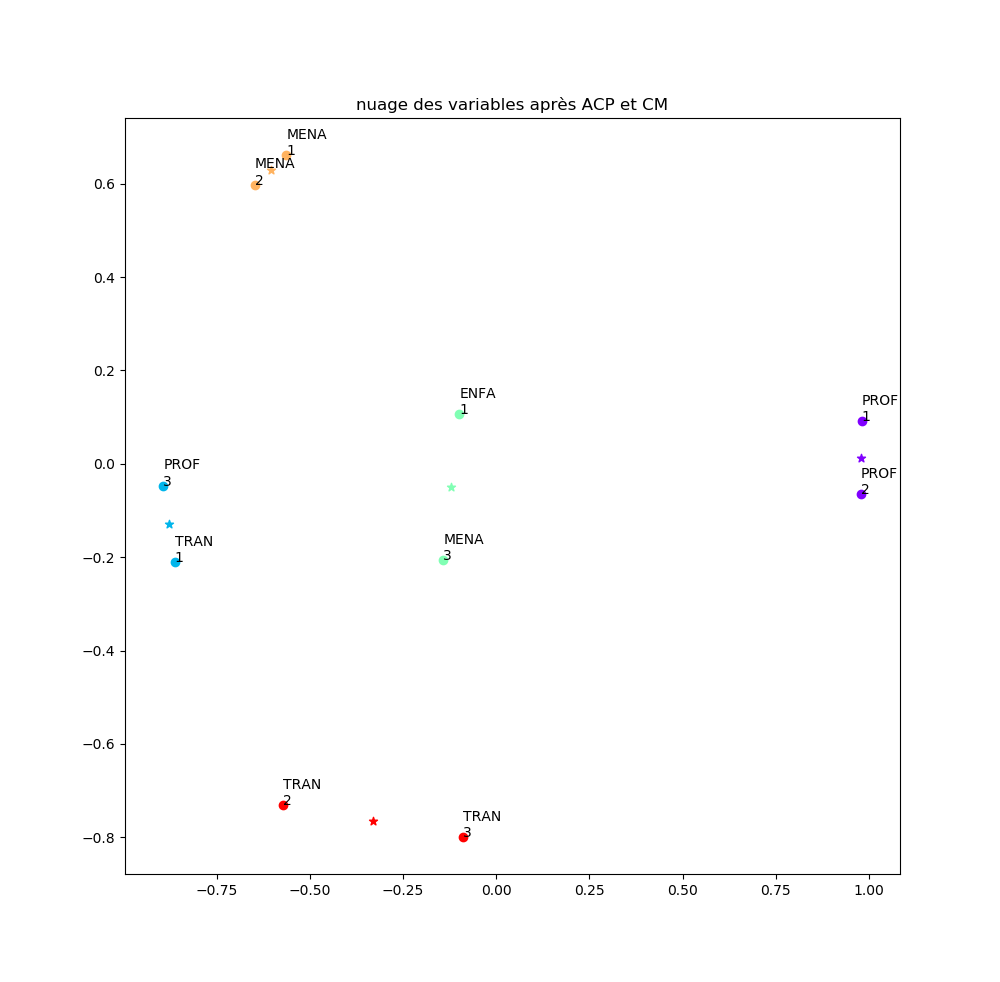
\includegraphics[width=0.9\textwidth]{img/Variables_ACP-CM.png}
            \caption{ACP + CM : Projection des variables}
            \label{Label_Variables_ACP-CM.png}
        \end{subfigure}
        \caption{Résultats pour l'ACP/ACM + CM : Projection des variables}
        \label{Label_Variables_ACP_ACM-CM.png}
    \end{figure}
    
\subsubsection{Commentaires et intérprétation}


On a observé ci dessus une classification satisfaisante des éléments, sans points aberrants. Cela permet dans l'exemple de données traité, de regrouper les métiers et occupations des individus en fonction du temps que cela leur prend, par exemple.

On peut néanmoins observer en appliquant plusieurs fois la méthodes, que la fonction place parfois un (ou plusieurs) centre isolé, ce qui rend une classe entière obsolète (cf. Figure \ref{fig: Label Classes_obsoletes_ACP-CM.png}.

%------ Pour insérer et citer une image centralisée -----
\insererfigure{img/Classes_obsoletes_ACP-CM.png}{8cm}{Cas des centres isolés}{Label Classes_obsoletes_ACP-CM.png}
% Le premier argument est le chemin pour la photo
% Le deuxième est la hauteur de la photo
% Le troisième la légende
% Le quatrième le label)

Dans l'exemple de résultat pour l'ACP ci-dessous, deux centres sur cinq ont été mal placés dans la représentation du nuage des individus. Il est à noter que cela n'implique pas un mauvais placement pour le nuage des variables. Cela montre une limitation de la méthode des centres mobiles, qui présente, due à son caractère aléatoire de placement de centres, des résultats parfois non conformes aux consignes, et nuisant à la bonne interprétation des données.

\subsection{ACP/ACM + Centres mobiles (CM)}
%METHODE DES CENTRES MOBILES (CM)

\subsubsection{Démarche}

La démarche pour les deux méthodes consiste à appliquer respectivement une ACP, après normalisation, et une ACM aux données, après mise en classe, puis de classer les résultats par une méthode des centres mobiles.

Les données utilisées dans l'exemple donné en graphique sont issues de la base "populations".

Ces données étant quantitatives, l'ACP peut s'appliquer directement, mais il faut réaliser une mise en classe pour obtenir un tableau disjonctif complet et réaliser l'ACM.

Une fois ces méthodes de factorisation appliquées, on peut appeler la fonction \textit{kmeans2} issue du module \textit{scipy.cluster.vq (K-means clustering and vector quantization)} pour réaliser une classification par la méthode des centres mobiles.

Dans les exemples de résultats ci-dessous, on a choisi respectivement un nombre de classes $k = 3$ et $5$ pour l'ACM et l'ACP arbitrairement en fonction du nombre de données pour obtenir des graphiques visibles tout en observant l'efficacité de la méthode.

Les étoiles représentent les centres, et les couleurs l'appartenance à la classe de chaque point.

    \begin{figure}[!htb]
        %\captionsetup[subfigure]{labelformat=empty}
        \begin{subfigure}[b]{0.48\textwidth}
            \centering
            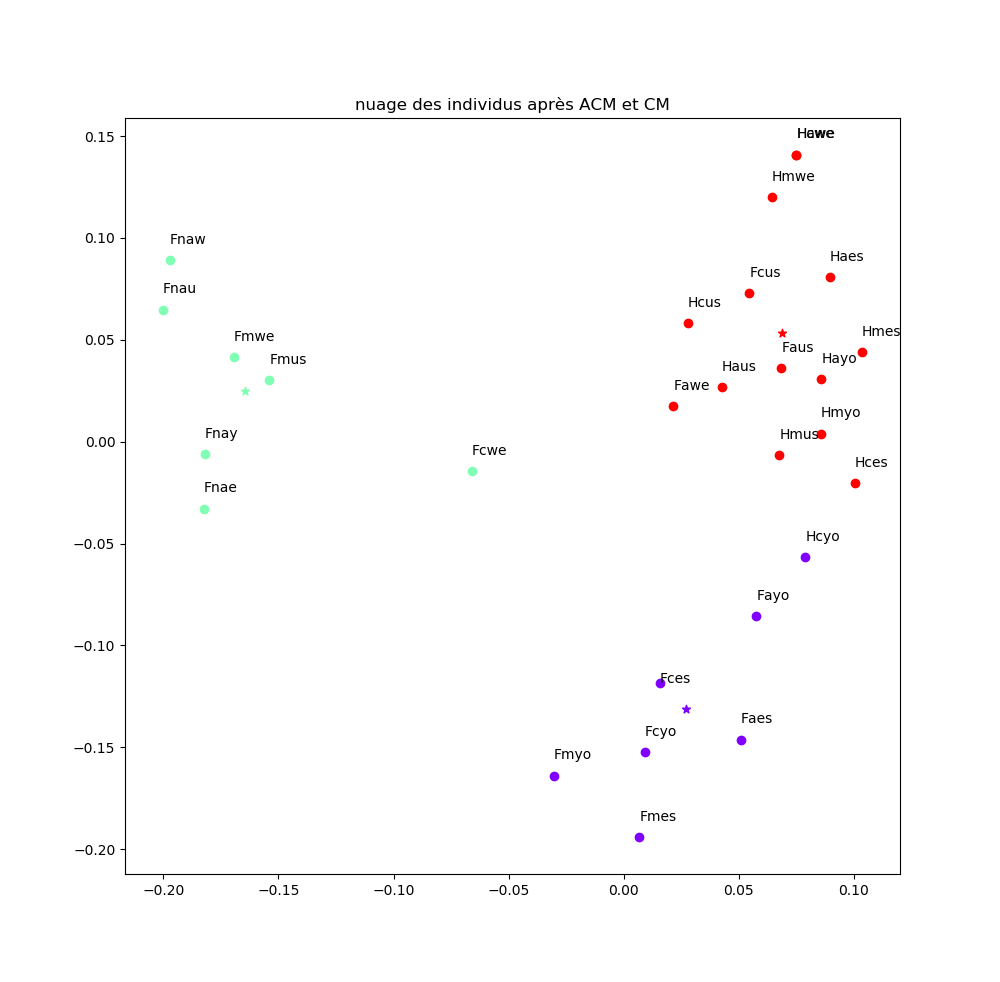
\includegraphics[width=0.98\textwidth]{img/Individus_ACM-CM.png}
            \caption{ACM + CM : Projection des individus}
            \label{Label_Individus_ACM-CM.png}
        \end{subfigure}
        \begin{subfigure}[b]{0.48\textwidth}
            \centering
            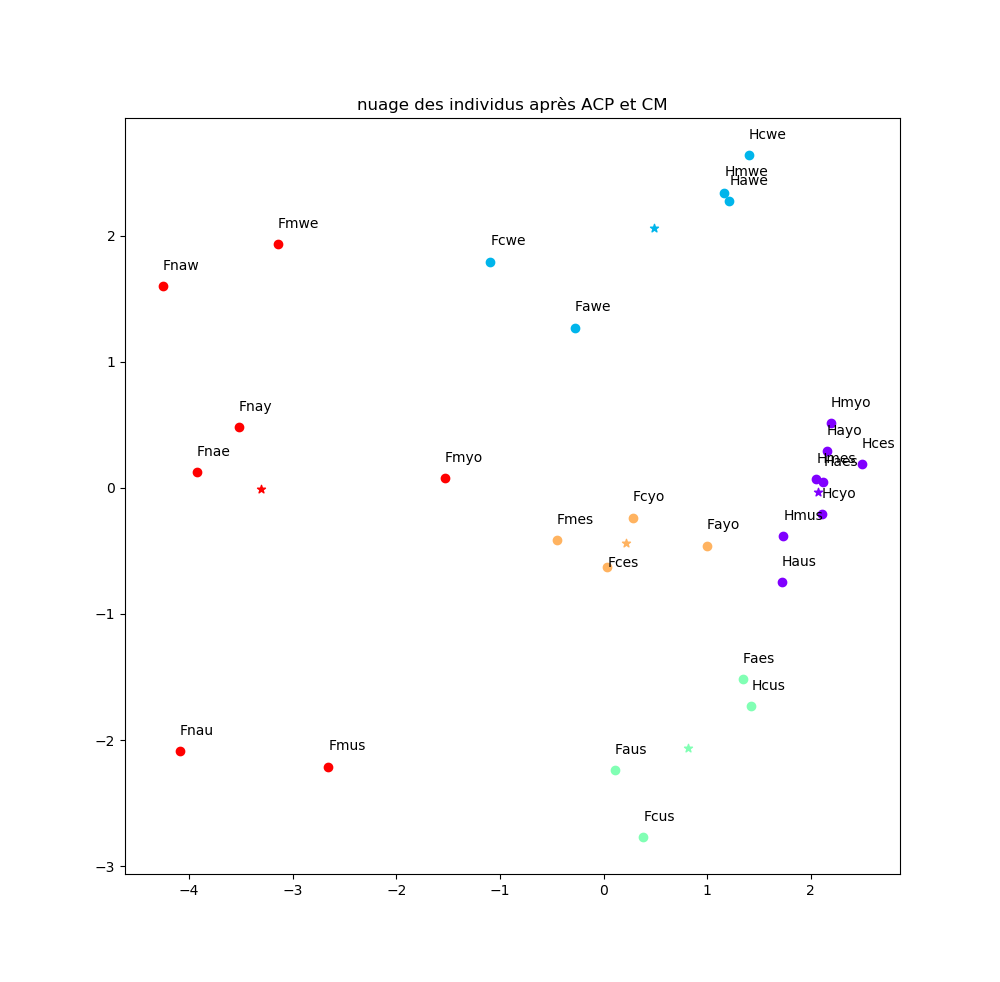
\includegraphics[width=0.98\textwidth]{img/Individus_ACP-CM.png}
            \caption{ACP + CM : Projection des individus}
            \label{Label_Individus_ACP-CM.png}
        \end{subfigure}
        \caption{Résultats pour l'ACP/ACM + CM : Projection des individus}
        \label{Label_Individus_ACP_ACM-CM.png}
    \end{figure}
    
    \begin{figure}[!htb]
        %\captionsetup[subfigure]{labelformat=empty}
        \begin{subfigure}[b]{0.48\textwidth}
            \centering
            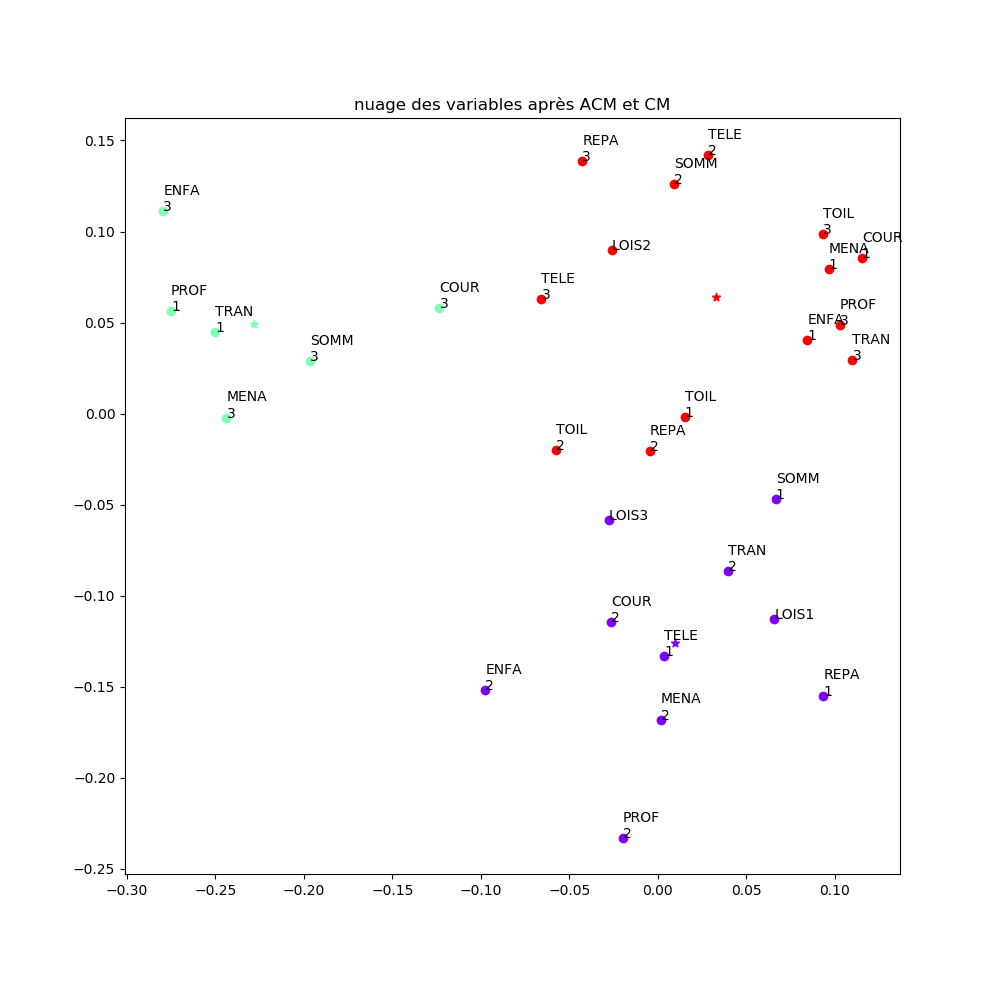
\includegraphics[width=0.98\textwidth]{img/Variables_ACM-CM.png}
            \caption{ACM + CM : Projection des variables}
            \label{Label_Variables_ACM-CM.png}
        \end{subfigure}
        \begin{subfigure}[b]{0.48\textwidth}
            \centering
            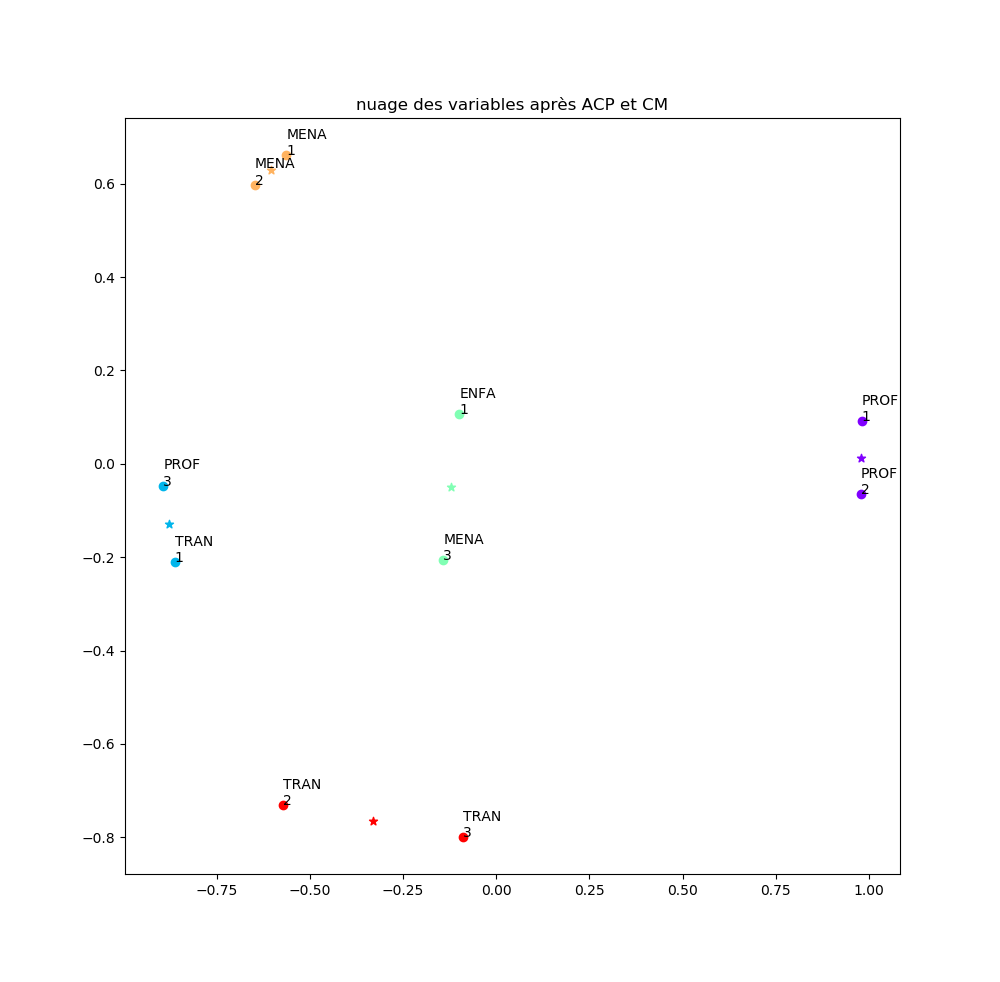
\includegraphics[width=0.98\textwidth]{img/Variables_ACP-CM.png}
            \caption{ACP + CM : Projection des variables}
            \label{Label_Variables_ACP-CM.png}
        \end{subfigure}
        \caption{Résultats pour l'ACP/ACM + CM : Projection des variables}
        \label{Label_Variables_ACP_ACM-CM.png}
    \end{figure}
    
\subsubsection{Commentaires et interprétation}


On a observé ci dessus une classification satisfaisante des éléments, sans points aberrants. Cela permet dans l'exemple de données traité, de regrouper les métiers et occupations des individus en fonction du temps que cela leur prend, par exemple.

On peut néanmoins observer en appliquant plusieurs fois la méthodes, que la fonction place parfois un (ou plusieurs) centre isolé, ce qui rend une classe entière obsolète (cf. Figure \ref{fig: Label Classes_obsoletes_ACP-CM.png}.

%------ Pour insérer et citer une image centralisée -----
\insererfigure{img/Classes_obsoletes_ACP-CM.png}{14 cm}{Cas des centres isolés}{Label Classes_obsoletes_ACP-CM.png}
% Le premier argument est le chemin pour la photo
% Le deuxième est la hauteur de la photo
% Le troisième la légende
% Le quatrième le label)

Dans l'exemple de résultat pour l'ACP ci-dessous, deux centres sur cinq ont été mal placés dans la représentation du nuage des individus. Il est à noter que cela n'implique pas un mauvais placement pour le nuage des variables. Cela montre une limitation de la méthode des centres mobiles, qui présente, due à son caractère aléatoire de placement de centres, des résultats parfois non conformes aux consignes, et nuisant à la bonne interprétation des données.



\section{Conclusion}
Nous avons, à travers cette étude, pu caractériser différentes méthodes de classifications et de factorisation d'un jeu de données. Si ces méthodes permettent toutes d'arriver à un même but, leur efficacité dépend de différents paramètres que nous avons mis en exergue, et elles ont toutes leurs limites. Ainsi, pour la méthode des centres mobiles,  nous avons vu que son utilisation de l'aléatoire pour placer les centres peut mener à une classification non conforme
aux consignes. Nous avons aussi vu que la méthodes CAH est très dépendante du calcul de distances utilisées.

De même, certaines méthodes de factorisation sont exclusive à des données quantitatives ou qualitatives, ce qui peut nécessiter un traitement de données au préalable. Toutes ces informations nous permettent de juger qu'aucune méthode n'est objectivement meilleure, mais qu'un choix judicieux des méthodes à appliquer est nécessaire au cas par cas pour obtenir un traitement de données adapté.

\newpage
\subsection{Code}

% \subsection{codage.py}
% \inputminted[linenos=True]{python}{scr/codage.py}

% \subsection{acp.py}
% \inputminted[linenos=True]{python}{scr/acp.py}

% \subsection{acm.py}
% \inputminted[linenos=True]{python}{scr/acm.py}

% \subsection{cah.py}
% \inputminted[linenos=True]{python}{scr/cah.py}

% \subsection{ACP + CAH}
% \inputminted[linenos=True]{python}{scr/mixte_acp_cah.py}

% \subsection{ACM + CAH}
% \inputminted[linenos=True]{python}{scr/mixte_acm_cah.py}

% \subsection{ACP + Centres mobiles}
% \inputminted[linenos=True]{python}{scr/ACP-CM.py}

% \subsection{ACM + Centres mobiles}
% \inputminted[linenos=True]{python}{scr/ACM-CM.py}

\newpage
\section{Annexe : abrégés des données « population »}

Les individus sont :
% https://www.tablesgenerator.com/
% https://support.office.com/fr-fr/article/combiner-le-texte-de-deux-cellules-ou-plus-en-une-cellule-81ba0946-ce78-42ed-b3c3-21340eb164a6
\begin{table}[h]
\centering
\begin{tabular}{|l|l|}
\hline
HAUS  & hommes actifs des USA                   \\ \hline
FAUS  & femmes actives des USA                  \\ \hline
FNAU  & femmes non actives des USA              \\ \hline
HMUS  & hommes mariés des USA                   \\ \hline
FMUS  & femmes mariées des USA                  \\ \hline
HCUS  & hommes célibataires des USA             \\ \hline
FCUS  & femmes célibataires des USA             \\ \hline
HAWE  & hommes actifs des pays de l'ouest       \\ \hline
FAWE  & femmes actives des pays de l'ouest      \\ \hline
FNAWE & femmes non actives des pays de l'ouest  \\ \hline
HMWE  & hommes mariés des pays de l'ouest       \\ \hline
FMWE  & femmes mariées des pays de l'ouest      \\ \hline
HCWE  & hommes célibataires des pays de l'ouest \\ \hline
FCWE  & femmes célibataires des pays de l'ouest \\ \hline
HAES  & hommes actifs des pays de l'est         \\ \hline
FAES  & femmes actives des pays de l'est        \\ \hline
FNAE  & femmes non actives des pays de l'est    \\ \hline
HMES  & hommes mariés des pays de l'est         \\ \hline
FMES  & femmes mariés des pays de l'est         \\ \hline
HCES  & hommes célibataires des pays de l'est   \\ \hline
FCES  & hommes célibataires des pays de l'est   \\ \hline
HAYO  & hommes actifs de Yougoslavie            \\ \hline
FAYO  & femmes actives de Yougoslavie           \\ \hline
HMYO  & hommes mariés de Yougoslavie            \\ \hline
FMYO  & femmes mariés de Yougoslavie            \\ \hline
FCYO  & femmes célibataires de Yougoslavie      \\ \hline
HCYO  & hommes célibataires de Yougoslavie      \\ \hline
\end{tabular}
\caption{signification des abrégés des données « population » : individus}
\label{tab:my-table}
\end{table}

Les variables sont :

\begin{table}[h]
\centering
\begin{tabular}{|l|l|}
\hline
PROF & travail professionnel                                          \\ \hline
TRAN & occupations dues ou liées au travail professionnel (transport) \\ \hline
MENA & travail ménager                                                \\ \hline
ENFA & occupations liées aux enfants                                  \\ \hline
COUR & les courses                                                    \\ \hline
REPA & les repas                                                      \\ \hline
SOMM & Sommeil                                                        \\ \hline
TELE & Télévision                                                     \\ \hline
LOIS & les autres loisirs                                             \\ \hline
\end{tabular}
\caption{signification des abrégés des données « population » : variables}
\label{tab:my-table2}
\end{table}

\end{document}